\documentclass[table]{beamer}
%[]中可以使用draft、handout、screen、transparency、trancompress、compress等参数

%指定beamer的模式与主题
\mode<presentation>
{
  \usetheme{Madrid}
%\usetheme{Boadilla}
%\usecolortheme{default}
%\usecolortheme{orchid}
%\usecolortheme{whale}
%\usefonttheme{professionalfonts}
}

%\usetheme{Madrid}
%这里还可以选择别的主题:Bergen, Boadilla, Madrid, AnnArbor, CambridgeUS, Pittsburgh, Rochester, Warsaw, ...
%有导航栏的Antibes, JuanLesPins, Montpellier, ...
%有内容的Berkeley, PaloAlto, Goettingen, Marburg, Hannover, ...
%有最小导航栏的Berlin, Ilmenau, Dresden, Darmstadt, Frankfurt, Singapore, Szeged, ...
%有章和节表单的Copenhagen, Luebeck, Malmoe, Warsaw, ...

%\usecolortheme{default}
%设置内部颜色主题(这些主题一般改变block里的颜色);这个主题一般选择动物来命名
%这里还可以选择别的颜色主题,如默认的和有特别目的的颜色主题default,structure,sidebartab,全颜色主题albatross,beetle,crane,dove,fly,seagull,wolverine,beaver

%\usecolortheme{orchid}
%设置外部颜色主题(这些主题一般改变title里的颜色);这个主题一般选择植物来命名
%这里还可以选择别的颜色主题,如默认的和有特别目的的颜色主题lily,orchid,rose

%\usecolortheme{whale}
%设置字体主题;这个主题一般选择海洋动物来命名
%这里还可以选择别的颜色主题,如默认的和有特别目的的颜色主题whale,seahorse,dolphin

%\usefonttheme{professionalfonts}
%类似的还可以定义structurebold,structuresmallcapsserif,professionalfonts

% 控制 beamer 的风格,可以根据自己的爱好修改
%\usepackage{beamerthemesplit} %使用 split 风格
%\usepackage{beamerthemeshadow} %使用 shadow 风格
%\usepackage[width=2cm,dark,tab]{beamerthemesidebar}

%插入音标
%\usepackage{tipa}
%\AtBeginDocument{
  %\renewcommand\textipa{\fontencoding{T3}\selectfont}
%}
%\AtBeginDocument{
  %\renewcommand\textipa[2][r]{{\fontfamily{cm#1}\tipaencoding #2}}
%}
%\renewenvironment{IPA}[1][r]
 %{\fontfamily{cm#1}\tipaencoding}
 %{}

% 设定英文字体
%\usepackage{fontspec}
% Fix bugs for fontspec in TeXLive2015
\ifdefined\suppressfontnotfounderror
  \expandafter\let\csname xetex_suppressfontnotfounderror:D\endcsname
    \suppressfontnotfounderror
\else
  \expandafter\let\csname xetex_suppressfontnotfounderror:D\endcsname
    \luatexsuppressfontnotfounderror
\fi
\usepackage[no-math]{fontspec}
\setmainfont{Times New Roman}
\setsansfont{Arial}
\setmonofont{Courier New}

% 设定中文字体
\usepackage[BoldFont,SlantFont,CJKchecksingle,CJKnumber]{xeCJK}
%\setCJKmainfont[BoldFont={Adobe Heiti Std},ItalicFont={Adobe Kaiti Std}]{Adobe Song Std}
\setCJKmainfont[BoldFont={Adobe Heiti Std},ItalicFont={Adobe Kaiti Std}]{WenQuanYi Micro Hei}
\setCJKsansfont{Adobe Heiti Std}
\setCJKmonofont{Adobe Fangsong Std}
\punctstyle{hangmobanjiao}

\defaultfontfeatures{Mapping=tex-text}
\usepackage{xunicode}
\usepackage{xltxtra}

\XeTeXlinebreaklocale "zh"
\XeTeXlinebreakskip = 0pt plus 1pt minus 0.1pt

\usepackage{setspace}
\usepackage{colortbl,xcolor}
\usepackage{hyperref}
%\hypersetup{xetex,bookmarksnumbered=true,bookmarksopen=true,pdfborder=1,breaklinks,colorlinks,linkcolor=blue,filecolor=black,urlcolor=cyan,citecolor=green}
\hypersetup{xetex,bookmarksnumbered=true,bookmarksopen=true,pdfborder=1,breaklinks,colorlinks,linkcolor=cyan,filecolor=black,urlcolor=blue,citecolor=green}

% 插入图片
\usepackage{graphicx}
\graphicspath{{figures/}}
% 图文混排
%\usepackage{picins}
\usepackage{floatflt}

% 可能用到的包
\usepackage{amsmath,amssymb}
%插入多媒体
%\usepackage{media9}
%\usepackage{movie15}
\usepackage{multimedia}
\usepackage{multicol}
\usepackage{multirow}

% 定义一些自选的模板,包括背景、图标、导航条和页脚等,修改要慎重
% 设置背景渐变由10%的红变成10%的结构颜色
%\beamertemplateshadingbackground{red!10}{structure!10}
%\beamertemplatesolidbackgroundcolor{white!90!blue}
% 使所有隐藏的文本完全透明、动态,而且动态的范围很小
\beamertemplatetransparentcovereddynamic
% 使itemize环境中变成小球,这是一种视觉效果
\beamertemplateballitem
% 为所有已编号的部分设置一个章节目录,并且编号显示成小球
\beamertemplatenumberedballsectiontoc
% 将每一页的要素的要素名设成加粗字体
\beamertemplateboldpartpage

% item逐步显示时,使已经出现的item、正在显示的item、将要出现的item呈现不同颜色
\def\hilite<#1>{
 \temporal<#1>{\color{gray}}{\color{blue}}
    {\color{blue!25}}
}

\renewcommand{\today}{\number\year 年 \number\month 月 \number\day 日}

%五角星
\usepackage{MnSymbol}

%去除图表标题中的figure等
\usepackage{caption}
\captionsetup{labelformat=empty,labelsep=none}

\usepackage{tabu}
\usepackage{multirow}
%表格自动换行
\usepackage{tabularx} 

% 千分号
%\usepackage{textcomp}

%罗马数字
\makeatletter
\newcommand{\rmnum}[1]{\romannumeral #1}
\newcommand{\Rmnum}[1]{\expandafter\@slowromancap\romannumeral #1@}
\makeatother

%分栏
\usepackage{multicol}

%\usepackage{enumitem}
%\usepackage{enumerate}

%键盘
\usepackage{keystroke}

%心形
%\usepackage{fdsymbol}

%插入源代码
\usepackage{listings}
\lstset{
  language=perl,                  % 程序语言名称:TeX, Perl, R, sh, bash, Awk
  basicstyle=\normalsize\tt,      %\tt指monospace字体族,程序源代码使用此族字体表示更加美观
  numbers=left,                   % 行号位置(左侧)
  numberstyle=\small,             % 行号字体的字号
  stepnumber=1,                   % 行号的显示步长
  numbersep=5pt,                  % 行号与代码间距
  backgroundcolor=\color{white},  % 背景色;需要 \usepackage{color}
  showspaces=false,               % 不显示空格
  showstringspaces=false,         % 不显示代码字符串中的空格标记
  showtabs=false,                 % 不显示 TAB
  tabsize=4, 
  frame=shadowbox,                % 把代码用带有阴影的框圈起来
  captionpos=b,                   % 标题位置
  breaklines=true,                % 对过长的代码自动断行
  breakatwhitespace=false,        % 断行只在空格处
  extendedchars=false,            % 解决代码跨页时,章节标题,页眉等汉字不显示的问题
  %escapeinside={\%*}{*},         % 跳脱字符,添加注释,暂时离开 listings 
  %escapeinside=``,
  commentstyle=\color{red!50!green!50!blue!50}\tt,  %浅灰色的注释
  rulesepcolor=\color{red!20!green!20!blue!20},     %代码块边框为淡青色
  keywordstyle=\color{blue!70}\bfseries\tt,         %代码关键字的颜色为蓝色,粗体
  identifierstyle=\tt,
  stringstyle=\tt,                % 代码字符串的特殊格式
  keepspaces=true,
  breakindent=1em,
  %breakindent=22pt,
  %breakindent=4em,
  breakautoindent=true,
  flexiblecolumns=true,
  aboveskip=1em,                  %代码块边框
  xleftmargin=2em,
  xrightmargin=2em
}

%\setbeamercolor{alerted text}{fg=magenta}
\setbeamercolor{bgcolor}{fg=yellow,bg=cyan}
%\setbeamercolor{itemize/enumerate body}{fg=green}

\begin{document}

%\includeonlyframes{current}

\logo{
\includegraphics[height=0.08\textwidth]{qr.png}}

% 在每个Section前都会加入的Frame
\AtBeginSection[]
{
  \begin{frame}<beamer>
    %\frametitle{Outline}
    \frametitle{教学提纲}
    \setcounter{tocdepth}{3}
    \begin{multicols}{2}
      \tableofcontents[currentsection,currentsubsection]
      %\tableofcontents[currentsection]
    \end{multicols}
  \end{frame}
}
% 在每个Subsection前都会加入的Frame
\AtBeginSubsection[]
{
  \begin{frame}<beamer>
%%\begin{frame}<handout:0>
%% handout:0 表示只在手稿中出现
    \frametitle{教学提纲}
    \setcounter{tocdepth}{3}
    \begin{multicols}{2}
    \tableofcontents[currentsection,currentsubsection]
    \end{multicols}
%% 显示在目录中加亮的当前章节
  \end{frame}
}

% 为当前幻灯片设置背景
%{
%\usebackgroundtemplate{
%\vbox to \paperheight{\vfil\hbox to
%\paperwidth{\hfil\includegraphics[width=2in]{tijmu_charcoal.png}\hfil}\vfil}
%}
\begin{frame}[plain]
  \begin{center}
    {\Huge 疯狂的实验\\}
    \vspace{1cm}
    {\LARGE 天津医科大学\\}
    %\vspace{0.2cm}
    {\LARGE 生物医学工程与技术学院\\}
    \vspace{1cm}
    {\large 2018-2019学年下学期(春)\\ 公共选修课}
  \end{center}
\end{frame}
%}



%\includeonlyframes{current}

\title[心理学与社会学]{第二章\quad 疯狂的实验——心理学与社会学}
\author[Yixf]{伊现富(Yi Xianfu)}
\institute[TIJMU]{天津医科大学(TIJMU)\\ 生物医学工程与技术学院}
\date{2017年2月}

\begin{frame}
  \titlepage
\end{frame}

\begin{frame}[plain,label=current]
  \frametitle{教学提纲}
  \setcounter{tocdepth}{3}
  \begin{multicols}{2}
    \tableofcontents
  \end{multicols}
\end{frame}


\begin{frame}
  \frametitle{心理学 | 小测验}
  \begin{figure}
    \centering
    
\includegraphics[width=0.6\textwidth]{c2.test.01.jpg}
  \end{figure}
\end{frame}

% 1-33,1883
\section{林格尔曼效应}
\begin{frame}
  \frametitle{林格尔曼效应}
  \begin{figure}
    \centering
    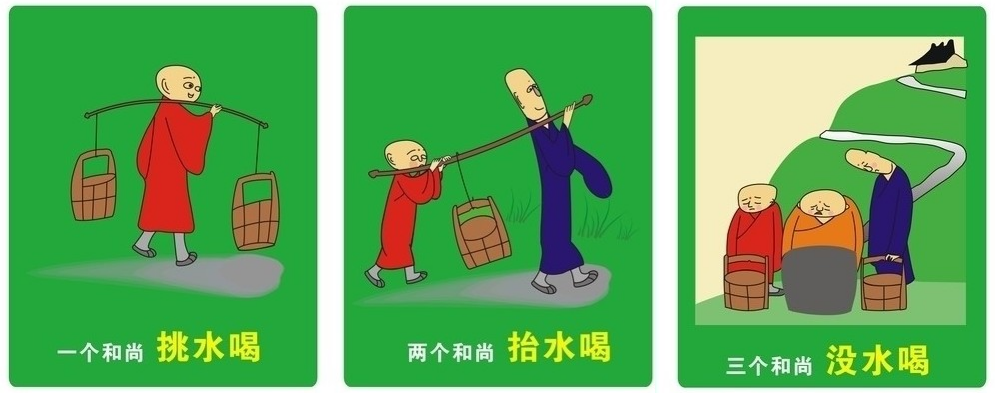
\includegraphics[width=\textwidth]{c2.ringelmann.01.png}
  \end{figure}
\end{frame}

\begin{frame}
  \frametitle{林格尔曼效应 | 实验}
  \begin{block}{实验设计}
      20名学生,分别独自和分组拽拉一根5米长的绳子,绳子的末端与测力器相连
  \end{block}
  \pause
  \begin{block}{实验结果}
    \begin{itemize}
      \item 2个人,平均每个人仅提供自己单独拉绳子时所用力的93\%
      \item 3个人,85\%
      \item 4个人,77\%
      \item 8个人,50\%
    \end{itemize}
  \end{block}
  \pause
  \begin{block}{实验解释}
    \begin{itemize}
      \item 社会性懒惰导致效率降低
      \item 小组中同步拽拉绳子有困难
    \end{itemize}
  \end{block}
\end{frame}

\begin{frame}
  \frametitle{林格尔曼效应 | 实验}
  \begin{block}{实验完善}
    \begin{itemize}
      \item 1人、2人、3人、4人、5人、6人、7人一组
      \item 每次实验中,只有一人毫不知情,其他人只是假装拽绳子
      \item 毫不知情的人在最前面,或者蒙上所有被试的眼睛
    \end{itemize}
  \end{block}
  \pause
  \begin{block}{结果确认}
    参与拉绳子的人越多,每个个体所出的力量越少。
  \end{block}
\end{frame}

\begin{frame}
  \frametitle{林格尔曼效应 | 总结}
  \begin{block}{林格尔曼效应}
    人是懒惰的,特别是在他认为别人没有注意到自己时。
  \end{block}
  \pause
  \begin{block}{效应解释}
    \begin{itemize}
      \item 在团队工作中,个人的努力并不明显影响总成绩,所以缺乏全力以赴的动力
      \item 个人的贡献看不出来,由此导致了人浮于事
    \end{itemize}
  \end{block}
  \pause
  \begin{block}{启示}
    \begin{itemize}
      \item 团队合作、项目管理
      \item 分工细致、责任明确
    \end{itemize}
  \end{block}
\end{frame}

% 2-99,1954
\section{调解冲突}
\begin{frame}
  \frametitle{调解冲突 | 实验}
  \begin{block}{问题}
    不同团体间的冲突。(先让2组男孩互相敌对,再完成一个看似不可能的任务:让斗得不可开交的11岁少年彼此和好。)
  \end{block}
  \pause
  \begin{block}{罗伯斯山洞实验(1954年)}
    \begin{itemize}
      \item 2组11岁的男孩,每组11人,素不相识,身世背景基本一致,“三好学生”
        \begin{itemize}
          \item 在操场上偷偷观察学生
          \item 与家长、老师攀谈,进一步证实判断
          \item 打探“房子多大”、“开什么车”之类的问题
        \end{itemize}
      \item 实验(3个阶段)
        \begin{enumerate}
          \item 各自独立、互不影响地生成2个团体
          \item 让2个团体有所接触,并为他们制造紧张氛围
          \item 尝试消除紧张氛围
        \end{enumerate}
      \item 使用2个已经成形的团队:已经成形的团队在面对其他团体时早就有了固定的行为方式?(这将破坏实验结果的真实性!)
    \end{itemize}
  \end{block}
\end{frame}

\begin{frame}
  \frametitle{调解冲突 | 结果}
  \begin{block}{实验结果}
    \begin{itemize}
      \item 第一阶段
    \begin{itemize}
      \item 取名字:“响尾蛇”,“老鹰”
      \item 建立了完善稳固的内部等级制度,形成了特色鲜明的集体行为方式:响尾蛇队爱说脏话,老鹰队爱裸泳
    \end{itemize}
      \item 第二阶段
    \begin{itemize}
      \item 尚未正式碰面,只是听说了对方的存在,就已经出言不逊了
      \item 4天时间,15场比赛,根据双方表现评分,奖品是梦寐以求的多功能组合军刀
      \item 互相谩骂、烧毁战旗、偷袭营地、寻仇报复、……
    \end{itemize}
      \item 第三阶段
    \begin{itemize}
      \item 让2组在非比赛、非敌对的氛围(看电影、吃饭)中会面——最终演变成一场互扔食物大战
      \item 给孩子们布置一些仅靠一队无法完成的任务(堵塞供水管道,“电影之夜”租金,推车搭帐篷)
      \item 短暂的和平(互借工具、共同劳作)——达成一致——最终和解(互借材料、分配食物、“毕营晚会”、同坐一辆车、分享牛奶)
    \end{itemize}
    \end{itemize}
  \end{block}
\end{frame}

\begin{frame}
  \frametitle{调解冲突 | 启示}
  \begin{block}{启示}
    \begin{itemize}
      \item 比赛可以增进团体内部的团结、引发对对方团体的鄙视和反感。
      \item 紧靠单纯的“接触”不足以平息争端;旧的冲突的解决,只能依靠新的冲突的产生。
      \item 更高级别的目标能够产生促进和平的功效;然而其他一些因素可能会抹杀这一功效。
    \end{itemize}
  \end{block}
\end{frame}

% 2-223,1993
\begin{frame}
  \frametitle{调解冲突 | 和平计划}
  \begin{block}{“朴素实在论”}
    \begin{itemize}
      \item 每个人都相信:自己看到的就是事物真正的样子。我们的大脑具有一种既值得钦佩又自私自利的能力,总认为自身的感知和看法是准确、切合实际且不带偏见的。
      \item 观点相左的2个人相遇,将会引发一系列影响深远的后果。(别人也有和我自己一样的想法!无意识“贬低”!)
    \end{itemize}
  \end{block}
  \vspace{-0.5em}
  \pause
  \begin{block}{实验}
    1993年以色列人和巴基斯坦人的和平提议,请一组学生作评价,一部分问卷对提议者进行调换
  \end{block}
  \vspace{-0.5em}
  \pause
  \begin{block}{内容 vs. 作者}
    \begin{itemize}
      \item 重要的不是提议的内容,而是提议的作者。
      \item 针对另一方的不可动摇的偏见为谈判造成了几乎无法克服的阻碍。
      \item 第三方的存在使双方接受和平计划的概率有了明显的提高。
    \end{itemize}
  \end{block}
\end{frame}

% 1-62,1904
\section{期望效应}
\begin{frame}
  \frametitle{期望效应 | 汉斯}
  \begin{block}{聪明的汉斯}
汉斯会做分数运算、数数、识图画、认时间、记日历,甚至还不时展示其音乐“造诣”(借助点头摇头、敲打马蹄的方式给出答案)
\vspace{-1em}
\begin{figure}
  \centering
  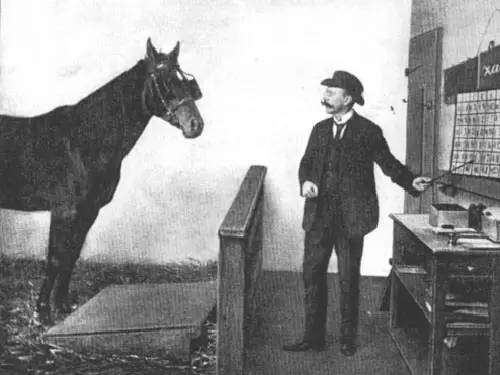
\includegraphics[width=0.35\textwidth]{c2.horse.01.jpg}\quad
  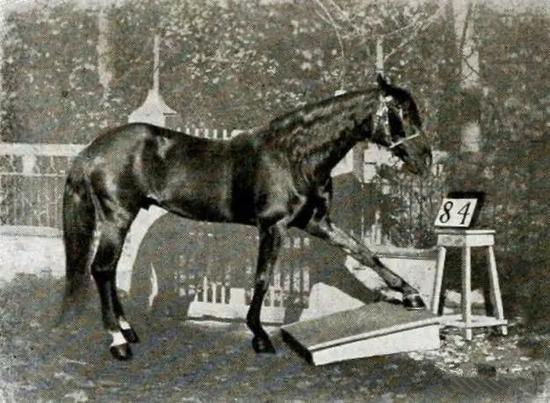
\includegraphics[width=0.36\textwidth]{c2.horse.02.jpg}\\
  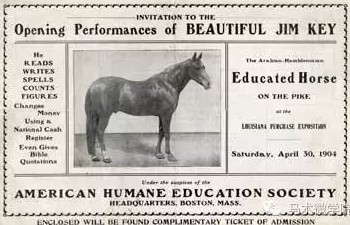
\includegraphics[width=0.4\textwidth]{c2.horse.03.jpg}
\end{figure}
  \end{block}
\end{frame}

\begin{frame}
  \frametitle{期望效应 | 汉斯}
  \begin{block}{舆论}
    \begin{itemize}
      \item (观众)汉斯与人唯一的区别就是无法言语
      \item (教育学家)汉斯的表现“达到了普通13-14岁小孩的智力水平”
      \item (动物学家)汉斯的表现证明了动物与人在灵魂层面并不存在区别
    \end{itemize}
  \end{block}
  \pause
  \begin{block}{汉斯委员会,鉴定书}
    \begin{itemize}
      \item 奥斯滕先生在汉斯的表演中没有作假
      \item 给汉斯的问题并非特意准备的
      \item “汉斯的表现,与以往任何表面与之相似的案例均存在本质的区别”
      \item “应当对这个现象进行严肃的、科学的调查”
    \end{itemize}
  \end{block}
\end{frame}

\begin{frame}
  \frametitle{期望效应 | 汉斯 | 实验一}
  \begin{block}{猜想}
  汉斯在回答问题时是否确实没有借助旁人的帮助?$\longrightarrow$实验者是否知晓答案对实验过程不会造成任何影响!
  \end{block}
  \pause
  \begin{block}{实验与结果}
    \begin{itemize}
      \item 任务:用马蹄按黑板上数字表明的次数敲打地面
      \item 两种方式分组实验:数字只给汉斯看(8\%)、将数字给汉斯和自己看(98\%)
      \item 只有汉斯知道答案:分别跟二人耳语一个数字,双方均不知道对方听到的数字(汉斯没能回答上来)
    \end{itemize}
  \end{block}
  \pause
  \begin{block}{结论}
    汉斯之所以能进行运算回答问题,是受了周围人群反应的暗示。
  \end{block}
\end{frame}

\begin{frame}
  \frametitle{期望效应 | 汉斯 | 实验二}
  \begin{block}{推理与假设}
    \begin{itemize}
      \item 在芬格斯特的实验过程中,冯\textbullet 奥斯滕根本不在现场!(无法通过各种途径向其提供暗示)
      \item 汉斯唯一可能的暗示来源,是实验者芬格斯特!(而芬格斯特对此一无所知)
    \end{itemize}
  \end{block}
  \pause
  \begin{block}{实验}
    \begin{itemize}
      \item 给汉斯带上眼罩
    \end{itemize}
  \end{block}
  \pause
  \begin{block}{结果与结论}
    \begin{itemize}
      \item 当汉斯看不见芬格斯特时,它再也回答不了问题。
      \item 汉斯确实是从提问者身上读出了答案。
    \end{itemize}
  \end{block}
\end{frame}

\begin{frame}
  \frametitle{期望效应 | 汉斯 | 实验三}
  \begin{block}{疑问与假设}
    \begin{itemize}
      \item 汉斯是如何从提问者身上读出答案的?
      \item 细致的观察后发现,汉斯是通过提问者身体的细微运动获取答案的提示!(提问—不自觉地微微低头—无意识地将目光从马蹄移开)
    \end{itemize}
  \end{block}
  \vspace{-0.4em}
  \pause
  \begin{block}{实验}
      在不同距离向汉斯提问;给汉斯提一些答案为1的问题;实验者未提任何问题但身体稍稍前倾
  \end{block}
  \vspace{-0.4em}
  \pause
  \begin{block}{结果}
    \begin{itemize}
      \item 与提问者的距离越远,汉斯的答案越不准确(越难看清提问者的身体动作)
      \item 对于答案为1的问题,汉斯要花费更大的精力(提问者下意识提示汉斯开始击蹄和结束击蹄的时间近乎一致,汉斯很难区分)
      \item 未提问而身体稍稍前倾时,汉斯一样会开始敲打马蹄
    \end{itemize}
  \end{block}
\end{frame}

\begin{frame}
  \frametitle{期望效应 | 汉斯 | 实验四}
  \begin{block}{验证}
    验证芬格斯特的推论。
  \end{block}
  \pause
  \begin{block}{实验}
    \begin{itemize}
      \item 25个人作为被试
      \item 芬格斯特要求他们在心中任意挑选一个数字
      \item 芬格斯特通过敲打桌子的方式猜测数字
    \end{itemize}
  \end{block}
  \pause
  \begin{block}{结果}
    芬格斯特成功猜中了23人心中的数字!
  \end{block}
\end{frame}

\begin{frame}
  \frametitle{期望效应 | 启示}
  \begin{block}{结局}
    \begin{itemize}
      \item 在《聪明的汉斯》一书后,芬格斯特再也没写过任何著作,发表的文章也寥寥无几。
      \item 冯\textbullet 奥斯滕失去了一切。
      \item 第一次世界大战期间,汉斯被征召入伍。
    \end{itemize}
  \end{block}
  \pause
  \begin{block}{期望效应(聪明的汉斯现象)}
    研究者在潜意识中希望实验朝着自己事先设想的方向发展,这种期望会不自觉地影响实验结果。
  \end{block}
  \pause
  \begin{block}{启示}
    \begin{itemize}
      \item 最能误导实验结果的一大因素:实验者的心理期望
      \item 在设计实验时,要充分考虑这一效应的影响
    \end{itemize}
  \end{block}
\end{frame}

% 1-130,1950
\section{囚徒困境}
\begin{frame}
  \frametitle{囚徒困境 | 实验}
  \begin{figure}
    \centering
    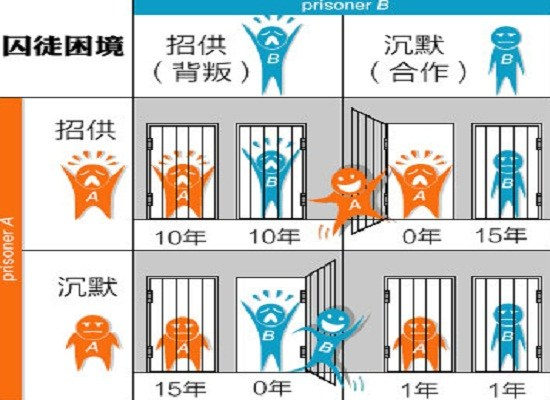
\includegraphics[width=0.8\textwidth]{c2.prisoner.01.jpg}
  \end{figure}
\end{frame}

\begin{frame}
  \frametitle{囚徒困境 | 策略}
  \begin{block}{博弈论中冲突的有趣之处}
    \begin{itemize}
      \item 在公开心中答案那一瞬间,没人知道对方的答案,但是最终的结果却取决于双方答案的契合度。
      \item 表面上最佳的理性选择最后会导致一个荒谬的结果:双方每个回合都选择“不合作”。
      \item 从严格意义上讲,囚徒困境是无法解答的,但利用博弈论,可以精确描述冲突与竞争,并为之提供相应的策略。
    \end{itemize}
  \end{block}
  \vspace{-0.3em}
  \pause
  \begin{block}{策略}
    \begin{itemize}
      \item 如果与博弈的对手只交锋一次,那么“不合作”无疑是最好的选择。否则,便不能如此。
      \item “以牙还牙”策略:第一回合“合作”,从第二回合起,与对方上一回的举动保持一致。
      \item 完善后的策略:如果有人欺骗了你,立刻还击。然而就此原谅对手,重新释放合作的善意。
    \end{itemize}
  \end{block}
\end{frame}

\begin{frame}
  \frametitle{囚徒困境 | 启示}
  \begin{block}{囚徒困境}
    囚徒困境(Prisoner's Dilemma)反映个人最佳选择并非团体最佳选择。或者说在一个群体中,个人做出理性选择却往往导致集体的非理性。
  \end{block}
  \pause
  \begin{block}{启示}
    \begin{itemize}
      \item 信任 vs. 欺骗 
      \item 个体 vs. 集体
    \end{itemize}
  \end{block}
  \pause
  \begin{block}{实例}
    \begin{itemize}
      \item 政治学——军备竞赛
      \item 经济学——关税战
      \item 商业——广告战
      \item 体育竞技——自行车赛
      \item ……
    \end{itemize}
  \end{block}
\end{frame}

% 1-203,1969
% 2-278,2005
\section{破窗理论}
\begin{frame}
  \frametitle{破窗理论 | 初始发现 | 实验}
  \vspace{-0.5em}
  \begin{block}{现象}
一天时间内,从工作地布朗克斯区的纽约大学到住处布鲁克林区218号共30公里长的线路上,心理学家菲利普\textbullet 津巴多发现不少辆遭受破坏的汽车。——这些破坏背后隐藏着什么?
  \end{block}
  \pause
  \begin{block}{实验(1969年)}
    \begin{itemize}
      \item 纽约布朗克斯区:已经使用10年的奥兹莫比尔车,停在校区对面,摘除号码牌、发动起引擎
      \item 加州帕洛阿尔托区:摘去牌号、引擎开动的汽车$\longrightarrow$抡起大锤砸车
    \end{itemize}
  \end{block}
  \begin{block}{结果}
    \begin{itemize}
      \item 10分钟后,第一批偷盗者(3人)
      \item “23起破坏性接触事件”
      \item 不到3天时间汽车变成一堆废铁
    \end{itemize}
  \end{block}
\end{frame}

\begin{frame}
  \frametitle{破窗理论 | 初始发现 | 结论}
  \begin{block}{破坏行动的基本模式}
    \begin{enumerate}
      \item 那些仍然可用或者可卖的东西会被首先偷走
      \item 当再没剩下什么有价值的东西可拿时,孩童和青少年会占领汽车,打破头灯及玻璃
      \item 接下来陆续有人使用石头、锤子和钢管来搞破坏,最终使汽车变成一堆垃圾
    \end{enumerate}
  \end{block}
  \pause
  \begin{block}{结论}
    \begin{itemize}
      \item 破坏行为的发生需要促发因素。
      \item 破坏行为就在光天化日众目睽睽之下发生。(常有路人围观破坏者)
      \item 夜幕的保护或者群体行动中个人的隐匿感显然是唤醒沉睡破坏力的必要条件。
      \item 大城市的规模和人口、嘈杂和喧嚣会造成人的隐匿感,加上衰败迹象遍布于没落街区,这些共同成为破坏行为的诱因。
    \end{itemize}
  \end{block}
\end{frame}

\begin{frame}
  \frametitle{破窗理论 | 初始发现 | 启示}
  \begin{block}{破窗理论}
诸如涂鸦、搞破坏、随地乱扔垃圾之类看似无害的违规做法将会引起极为严重的犯罪行为,因为它会给人造成一种印象,即“事态已经失去控制,谁也不会因为任何事情被追究责任”。
  \end{block}
  \pause
  \begin{block}{启示}
    \begin{itemize}
      %\item 衰败坍塌的迹象会增强人们进行破坏性行为的意愿,不仅那些被拆毁的汽车会“勾引”人们“为非作歹”,其他各类残破景象都能产生这种效果。
    \item 破坏行为的发生需要促发因素。“仅仅一片没有更换的破玻璃也是一个强大信号,暗示无人管理、打碎玻璃不用承担后果”。$\Longrightarrow$ 最好在混乱情况初露端倪时就消灭它。$\Longrightarrow$ 破罐子破摔 $\Longrightarrow$ 勿以恶小而为之,勿以善小而不为
      \item 一些很不起眼的小事物往往造成人的不安,比如涂鸦、街道上的废弃物、破坏行为。这些事物在人的内心造成一种感觉,似乎形势已经不受控制,谁也不必为什么负责。$\Longrightarrow$ 通过克服杂乱无序的外部特征就可以减少犯罪几率。?
    \end{itemize}
  \end{block}
\end{frame}

\begin{frame}
  \frametitle{破窗理论 | 初始发现 | 应用}
  \begin{block}{应用}
    \begin{itemize}
      \item 20世纪90年代,纽约,警察总长比尔\textbullet 布拉顿
      \item 画有涂鸦的地铁列车马上停止运行并接受清洗,醉酒者和行乞者遭到驱赶,垃圾被打扫干净
      \item 自1994年任职以来,纽约的谋杀率降低了将近一半(成果源于“零容忍政策?仍有争议!)
    \end{itemize}
  \end{block}
\end{frame}

\begin{frame}
  \frametitle{破窗理论 | 深入研究 | 实验一}
  \begin{block}{问题}
    \begin{itemize}
      \item 破窗理论过于笼统,且并未在普遍事实中得到检验。
      \item 还没有人做过严谨、正规的科学研究:“主观意图中无伤大雅的违规行为”应该作何解释?这种违规行为对他人违法的促进作用到底有多强?
    \end{itemize}
  \end{block}
  \pause
  \begin{block}{实验一(2005年)}
    \begin{itemize}
      \item 把整条胡同(有个自行车停车场,没有垃圾桶)刷成灰色,立一块”禁止涂鸦“的牌子 $\rightarrow$ 第二天,在每辆自行车车把上放一张传单
      \item 在胡同外墙上涂鸦(足够空洞无聊,不会被当做艺术品) $\rightarrow$ 第二天,在车把上放传单
    \end{itemize}
  \end{block}
  \pause
  \begin{block}{结果}
    把传单扔到地上的人:33\% $\rightarrow$ 69\%
  \end{block}
\end{frame}

\begin{frame}
  \frametitle{破窗理论 | 深入研究 | 实验一 | 启示}
  \begin{block}{启示}
对一种规范的破坏(禁止涂鸦)促进了对另一种规范(不应随地乱丢垃圾)的破坏;破坏规范的行为好像一种传染病,能够传染人们破坏其他的规范。
  \end{block}
  \pause
  \begin{block}{“目标框架理论”}
    指导人类行为的“目标”无外乎以下3种:
    \begin{enumerate}
      \item 规范向导:我要做得体的事。
      \item 享受向导:我要做让我感觉良好的事,比如不太费力的事。
      \item 利益向导:我要做能够改善我的物质处境的事。
    \end{enumerate}
    这些目标之间经常存在竞争关系,它们的优先级可能由于某个外部事件而发生改变。
  \end{block}
\end{frame}

\begin{frame}
  \frametitle{破窗理论 | 深入研究 | 实验二}
  \begin{block}{实验二(2005年)}
    \begin{itemize}
      \item 用活动栅栏封住医院停车场的入口,只留下50厘米宽的通道;在栅栏上固定2块禁令牌:“禁止用链子栓自行车”和“禁止横穿,请走侧面入口” $\rightarrow$ 在栅栏上栓上/不栓4辆自行车 $\rightarrow$ 从“禁行通道”中挤过去的行人:82\% vs. 27\%
      \item 自行车主听到有人在自行车停车场附近违反禁令、燃放烟花爆竹,他们随地扔掉传单的概率也会比没有感知到破坏规范时增加30\%。
    \end{itemize}
  \end{block}
  \pause
  \begin{block}{启示}
    \begin{itemize}
      \item 对第一条规范的破坏导致对第二条规范的破坏。个人订立的规则也服从这一效应。
      \item 即使破坏规范的行为不是从视觉上感知到的,“不良行径”照样会蔓延。
    \end{itemize}
  \end{block}
\end{frame}

\begin{frame}
  \frametitle{破窗理论 | 深入研究 | 实验三}
  \begin{block}{疑问}
 对无关紧要的规则加以破坏也会导致事关重大的社会规范受到冲击吗? 
  \end{block}
  \pause
  \begin{block}{实验三(2005年):“唆使”人们偷东西}
    \begin{itemize}
      \item 往一个信封里放入5欧元纸币(复印出来的伪钞),让它通过信封的“透明窗口”显露出来,并将信封半塞进一个邮筒里
      \item 在邮筒上喷绘涂鸦 vs. 在邮筒周围撒一些垃圾 vs. 到处干干净净
    \end{itemize}
  \end{block}
  \pause
  \begin{block}{结果}
    偷钱的人数:邮筒干净时13\%,其他2种情况下翻一倍
  \end{block}
\end{frame}

\begin{frame}
  \frametitle{破窗理论 | 深入研究 | 实验三 | 启示}
  \begin{block}{应用}
    \begin{itemize}
      \item 建议在阿姆斯特丹专门开放部分屋墙允许合法喷绘
      \item 阿姆斯特丹议会通过一项法律,规定每个涂鸦涂上之后必须立刻清除。
    \end{itemize}
  \end{block}
  \pause
  \begin{block}{告诫}
    \begin{itemize}
       \item  不要相信通过修补窗玻璃和粉刷墙壁就能使一个衰败的住宅区再次兴盛。
       \item 如果对规范的破坏早已进入那些并非公开可见的领域,那么在那些领域中,仅仅重新建立有形的秩序将会助益甚微。
    \end{itemize}
  \end{block}
\end{frame}

% 2-160,1969
\section{去个体化}
\begin{frame}
  \frametitle{去个体化 | 实验}
  \begin{block}{问题}
    \begin{itemize}
      \item 如果人们发现自己处于某个可以隐匿身份的群组,他们的行为会有何种变化?
      \item 由变装带来的匿名化效应是否推动了群组中攻击性的增长?
    \end{itemize}
  \end{block}
  \pause
  \begin{block}{实验室实验}
    \begin{itemize}
      \item 一群女性对另一个人进行电击,佩戴姓名标牌 vs. 伪装(面具+超大围裙)
      \item 伪装时实施电击的持续时间与没有伪装并且佩戴姓名标牌时相比,整整翻了一番!
    \end{itemize}
  \end{block}
\end{frame}

\begin{frame}
  \frametitle{去个体化 | 实验一}
  \begin{block}{万圣节实验——自然环境}
    \begin{itemize}
      \item 万圣节聚会,8项游戏(4种比较静态,4种强调对抗),赢取兑换券(聚会结束后换取玩具)
      \item 变装前——变装(单独的隔间、服饰看起来都一样)阶段——变装后,各一小时;黄色灯泡固定每20秒闪烁一次,与此同时,几名成年人观察记录,戴滤色镜观察斗篷上仅凭肉眼看不到的数字
    \end{itemize}
  \end{block}
  \pause
  \begin{block}{结果}
    \begin{itemize}
      \item 变装后一种攻击性的氛围迅速扩散开来(互相推撞、大喊大叫、彼此殴打)
      \item 本该持续一个小时的匿名阶段被提前终止
      \item 没有了变装服饰的孩子们立刻又平静下来
      \item 兑换券数量:58——31——79(与个体利益相悖,但攻击行为带来了“游戏的乐趣”)
    \end{itemize}
  \end{block}
\end{frame}

\begin{frame}
  \frametitle{去个体化 | 实验二}
  \begin{block}{万圣节实验}
    \begin{itemize}
      \item 27所房子同时进行,入口处看起来都一样:一张桌子上放着2只碗,一只装着糖果,60厘米外的另一只装着零钱
      \item 孩子们挨家挨户敲门讨糖,以为不认识的女士请他进门,并说“每个人都可以拿1块糖。我得回另一个房间干活去了。”
      \item 孩子们被单独留下,自由活动(实验助手藏在柜子里通过微小的窥视孔观察他们)
    \end{itemize}
  \end{block}
  \vspace{-0.5em}
  \pause
  \begin{block}{结果}
    \begin{itemize}
      \item 如果女士在离开房间前询问过孩子们的名字,只有21\%会去偷窃
      \item 如果孩子们保持匿名,比率变成57\%
      \item 如果女士对群组中的一个孩子单独强调“如果丢了什么东西的话,就是你的责任”,有80\%的孩子会去偷窃
      \item 如果来敲门的孩子是独自一人,即便没有被问到名字,也只有20\%会在未经允许的情况下去碗里抓东西
    \end{itemize}
  \end{block}
\end{frame}

\begin{frame}
  \frametitle{去个体化 | 启示}
  \begin{block}{启示}
    \begin{itemize}
      \item “去个体化”会导致身处群组中的人做出他们作为个体绝对不会做的事情来。
      \item 群组中的匿名性促进了攻击性;个体的匿名性影响则要小得多。
      \item 群组中的匿名性在现实中的重大违法犯罪行为(大屠杀、游行暴动等)中扮演决定性的角色。
      \item 匿名不仅可以使人免受惩罚,更可怕的是,它会使人失去自制力,最终迷失自我。这时,只要少数几个人迈出第一步,连锁反应就会开始。
    \end{itemize}
  \end{block}
\end{frame}

% 1-244,1973
\section{归因错觉}
\begin{frame}
  \frametitle{归因错觉}
  \begin{figure}
    \centering
    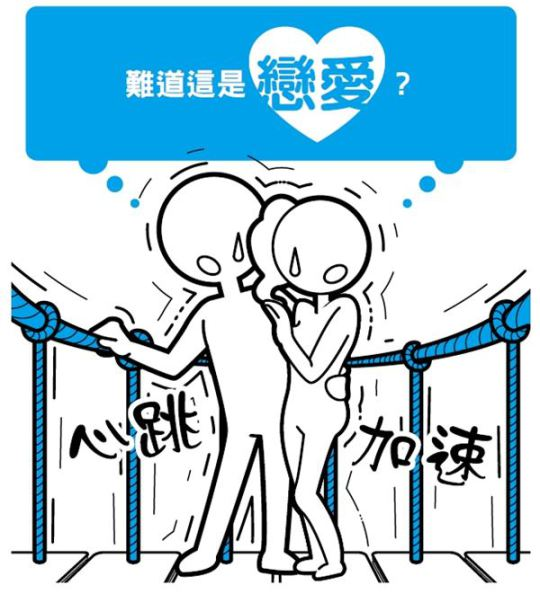
\includegraphics[width=0.4\textwidth]{c2.bridge.01.jpg}
    \visible<2->{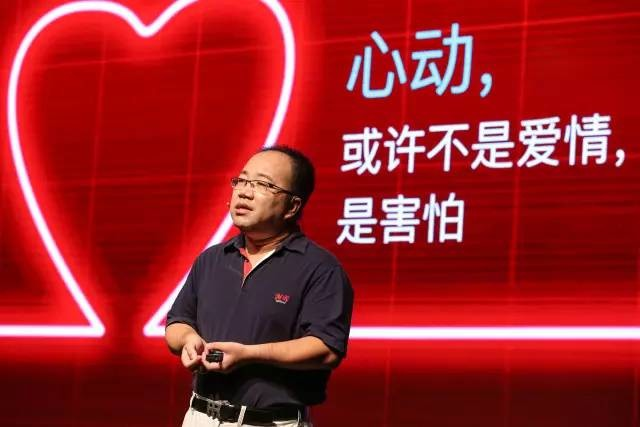
\includegraphics[width=0.55\textwidth]{c2.bridge.02.jpg}}
  \end{figure}
\end{frame}

\begin{frame}
  \frametitle{归因错觉 | 实验}
  \begin{block}{实验(1973年)}
    一位漂亮的女大学生,对男游客编一个谎话(问卷),然后留下姓名和电话:
    \begin{itemize}
      \item 从吊桥上走过、膝盖还在发抖的男游客
      \item 已经从吊桥上下来有一阵子的男游客
    \end{itemize}
  \end{block}
  \pause
  \begin{block}{结果}
    第二天,打电话联系女大学生的男游客:13/25 vs. 7/23
  \end{block}
  \pause
  \begin{block}{解释}
那些刚从吊桥上走下来的游客,错误地把膝盖的颤抖归因于看到格洛莉亚,所以他们中的相当部分会产生与格洛莉亚进一步接触的愿望。
  \end{block}
\end{frame}

\begin{frame}
  \frametitle{归因错觉 | 启示}
  \begin{block}{归因错觉}
    当人的身体受到特定的刺激的时候,这种身体的感觉会错误地被当成另外一种刺激。
  \end{block}
  \pause
  \begin{block}{启示}
父母如果禁止年轻人互相往来,就得避免给年轻人其他的刺激,因为那些刺激会被误理解为爱情造成的,从而让两个年轻人的心靠得更近。(罗密欧与朱丽叶)
  \end{block}
\end{frame}

% 2-91,1951
\section{从众心理}
\begin{frame}
  \frametitle{从众心理 | 阿希测试}
  \begin{figure}
    \centering
    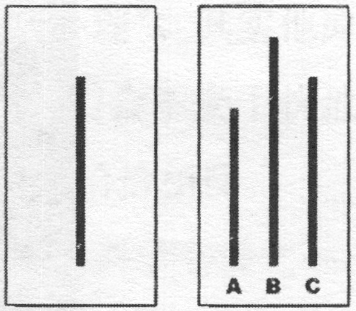
\includegraphics[width=0.7\textwidth]{c2.asch.01.png}
  \end{figure}
\end{frame}

\begin{frame}
  \frametitle{从众心理 | 实验}
  \begin{block}{问题}
    \begin{itemize}
      \item 人们是否容易屈从于集体的压力?
      \item (意欲证明)人们不会毫无主见地服从团体,人们会不受干扰地表达自己的观点。
    \end{itemize}
  \end{block}
  \pause
  \begin{block}{实验}
    \begin{itemize}
      \item 以前的实验:被试阅读同一段文章,判断作者(答案不是一清二楚的“对”或“错”)
      \item 判断线段长短:1951年,所罗门\textbullet 阿希,“阿希测试”(“从众测试”)
    \end{itemize}
  \end{block}
\end{frame}

\begin{frame}
  \frametitle{从众心理 | 实验}
  \begin{block}{从众测试}
    \begin{itemize}
      \item 2张画着线段的白板——2张——2张;5名被试(主持人的“同伙”)+ 6号被试者
      \item 5名被试:前两次说正确答案,最后一次统一说出错误答案;最后一次6号被试的答案是……
    \end{itemize}
  \end{block}
  \pause
  \begin{block}{结果}
    \begin{itemize}
      \item 追随集体意见、给出错误答案的比例高达1/3。
      \item 只有1/4的被试者一次都没有屈从于集体的压力。
    \end{itemize}
  \end{block}
\end{frame}

\begin{frame}
  \frametitle{从众心理 | 实验}
  \begin{block}{规律}
    \begin{itemize}
      \item 1966年,17个国家,133场从众实验:
    \begin{itemize}
      \item 如果冒牌被试者中多一个人报出正确答案,正牌测试者给出错误答案的比例就会从32\%降至5\%。(在团体中不同意见的重要性。)
      \item 如果被试者可以把答案写下来而不是当众说出来——尽管他有机会获悉别人的答案,追随他人意见的比例也会大大降低。
    \end{itemize}
      \item 不同时代、不同文化圈中开展“阿希实验”,得到不一样的结果:
        \begin{itemize}
      \item 在强调个性的西方发达国家,从众趋势相对较弱;在将集体利益置于个体利益之上的远东和非洲地区,从众的倾向极为明显。
      \item 自20实际50年代阿希首次实验至今,被试者产生从众行为的趋势正在逐渐减弱,但还没有完全消失。
        \end{itemize}
    \end{itemize}
  \end{block}
\end{frame}

\begin{frame}
  \frametitle{从众心理 | 启示}
  \begin{block}{启示}
    \begin{itemize}
      \item 阿希的“从众测试”是全世界被重复操作次数最多的科学实验之一。
      \item 在很多时候,大部分人的意见才是对的,顾及他人感受也是通达人情的表现。
      \item 严肃对待别人说出的信息,并不一定代表无知。
      \item 被试者明知他人说错还要跟着说错,是为了保住他人的脸面。
      \item 跟风:笑话、鼓掌、……
    \end{itemize}
  \end{block}
\end{frame}

% 2-106,1956
\section{认知失调}
\begin{frame}
  \frametitle{认知失调 | 理论}
  \begin{block}{认知失调}
    当我们的想法和行为不一致时,或者当我们的2个想法互相矛盾时,内心会产生一种冲突。例如:
    \begin{itemize}
      \item 吸烟者明明了解吸烟的危害,却依然吸烟。
      \item 女人虽然知道名牌鞋子过于昂贵,却依然购买。
    \end{itemize}
  \end{block}
  \pause
  \begin{block}{假设}
    人们需要在行为和想法之间重建一致关系,以消除“认知失调”造成的压力,而重建一致关系的途径只有2个:
    \begin{enumerate}
      \item 改变行为
      \item 改变想法(如果人们不能或者不愿改变行为,那就只好对行为做出荒谬的辩解,甚至心甘情愿地相信这些辩解——吸烟根本没有那么大的危害,名牌鞋子的质量更胜一筹……)
    \end{enumerate}
  \end{block}
\end{frame}

\begin{frame}
  \frametitle{认知失调 | 吸烟}
  \begin{figure}
    \centering
    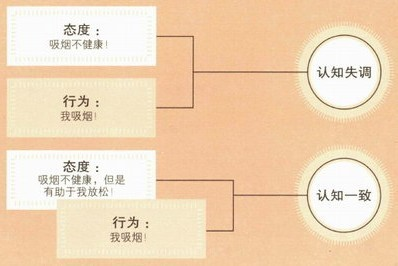
\includegraphics[width=0.8\textwidth]{c2.smoke.01.jpg}
  \end{figure}
\end{frame}

\begin{frame}
  \frametitle{认知失调 | 实验}
  \begin{block}{设想}
什么情况容易导致“认知失调”?——“接纳仪式”!(与轻松入组的成员相比,经过各种努力才艰难入组的成员更加觉得小组充满魅力?)
  \end{block}
  \vspace{-0.6em}
  \pause
  \begin{block}{科学验证——入组实验}
    \begin{itemize}
      \item 入组测试:21名年轻的女大学生,艰难的入组(朗读猥亵词语)
      \item 需要检验:与未参加测试或者只经历了简单测试的女生相比,这些通过艰难测试的女生是否更加看重自己的小组成员身份。
      \item 检验方法:实验参与者戴上耳机(单间、使用对讲机)倾听讨论组正在进行的谈话(不存在小组,播放事先录好的声音)
      \item 讨论内容:“要多没用就有多没用、要多无聊就有多无聊”
    \end{itemize}
  \end{block}
  \vspace{-0.6em}
  \pause
  \begin{block}{结果}
与其他人相比,通过尴尬测试的女生更加觉得讨论内容和谈话人员都很有趣(她们在用这种方式减轻“艰难的入组”与“无聊的讨论”之间的“失调”)。
  \end{block}
\end{frame}

\begin{frame}
  \frametitle{认知失调 | 启示}
  \begin{block}{普遍性与基本性}
    \begin{itemize}
      \item 3000多篇研究论文;从日常小事到世界政治,这一特质都在默默发挥自己的力量。
      \item 卷尾猴实验:起初并没有发现3种颜色有何区别,但偶然挑选黄色的糖豆后就会一直偏爱黄色。
    \end{itemize}
  \end{block}
  \pause
  \begin{block}{启示}
    \begin{itemize}
      \item 减轻“认知失调”是一个不自觉的过程,旁观者清,当局者迷。
      \item 减轻“认知失调”是一种应对生活的原始策略,它能消除内心矛盾,在愿望无法实现时调整情绪。(孩子会让我们幸福!?)
      \item 减轻“认知失调”往往也会引发糟糕的情况。(审判失误)
    \end{itemize}
  \end{block}
\end{frame}

% 2-112,1960
\section{选择任务}
\begin{frame}
  \frametitle{选择任务 | 四卡问题}
  \begin{block}{四卡问题}
    \begin{figure}
      \centering
      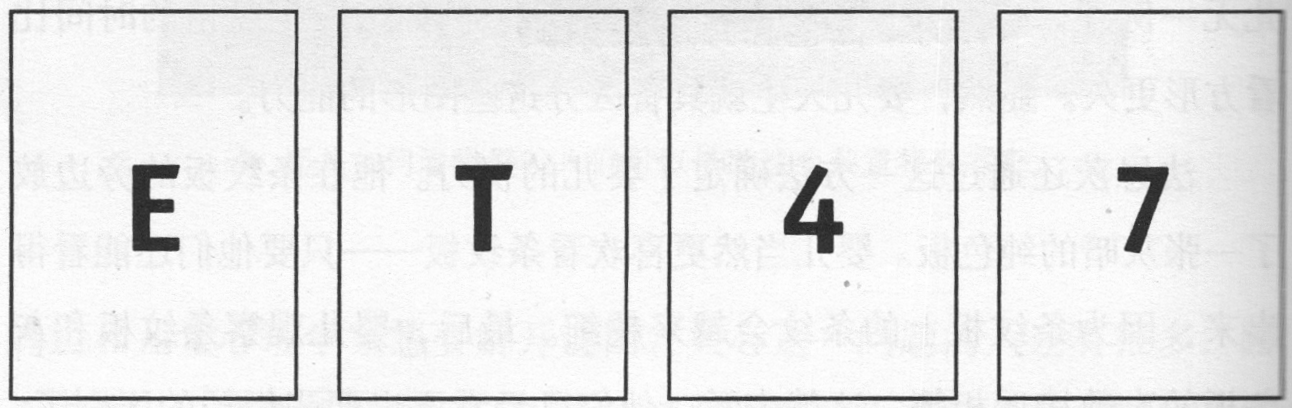
\includegraphics[width=0.9\textwidth]{c2.cards.01.png}
    \end{figure}
    若卡片一面为元音字母,则另一面为偶数。你必须翻看哪几张卡片,才能验出命题的真伪?
  \end{block}
\end{frame}

\begin{frame}
  \frametitle{选择任务 | 四卡问题 | 启示}
  \begin{block}{选择任务(selection task)}
 心理学界反复探讨的思维游戏,“道义逻辑思维与选择任务”、“沃森选择任务中的复杂问题效应”等上百项研究的中心议题。
  \end{block}
  \pause
  \begin{block}{结果}
    \begin{itemize}
      \item 只有不到10\%的被试者能够制定出正确的解决方案。
      \item 128名学生中:5人做对,59人表示需要翻转E和4,42人认为只需翻转E,其他人的答案更是五花八门。
    \end{itemize}
  \end{block}
  \pause
  \begin{block}{启示}
    \begin{itemize}
      \item 面对某种假设,人们往往会不自觉地收集更多信息去确认它,而不是推翻它。
      \item 习惯“证实”、不习惯“证伪”,似乎是某种根深蒂固的人性需求,正是由于它的驱动,人们才会狂热地信奉伪科学和阴谋论。
    \end{itemize}
  \end{block}
\end{frame}

% 2-130,1964
\section{旁观者效应}
\begin{frame}
  \frametitle{旁观者效应 | 缘起}
  \begin{block}{新闻报道}
    “女子在邱园惨遭非礼与刺杀,皇后区38位可敬的守法公民袖手旁观逾半小时。”——1964年3月27日,《纽约时报》(过度渲染的不实报道!)
  \end{block}
  \pause
  \begin{block}{假设}
    将某种集体行为归因于某个个体的病态性格是毫无道理可言的,这也许恰恰反映了某种正常的集体效应。包含2种可能性:
    \begin{enumerate}
      \item 责任分散:在场的“他人”越多,“我”的救援责任就越小。
      \item 错误定性:“他人”没有伸出援手,“他人”可能比“我”更了解情况,因此情况应该不太紧急。
    \end{enumerate}
  \end{block}
\end{frame}

\begin{frame}
  \frametitle{旁观者效应 | 启示}
  \begin{block}{实验}
    \begin{itemize}
      \item 检测“责任分散”:2人——85\%,52秒;3人——62\%,93秒;6人——31\%,2分多钟之后
      \item 检测“错误定性”:1人——3/4;3人——13\%
    \end{itemize}
  \end{block}
  \pause
  \begin{block}{启示}
    \begin{itemize}
      \item 针对“责任分散”——遇到危险的人应该怎样激醒他人“麻木迟钝”的本性?推荐受困者向一群人中的一个人求助!
      \item 针对“错误定性”——救生员绝对不能参照他人的反应做出判断,必须自行认定游泳者是真的陷入困境还是在嬉戏。
      \item 让更多的人了解实验——对实验早有耳闻的被试者面对紧急情况,做出积极反应的比率几乎达到普通被试者的2倍。
    \end{itemize}
  \end{block}
\end{frame}

% 2-170,1972
\section{安慰剂信息}
\begin{frame}
  \frametitle{安慰剂信息 | 观点}
  \begin{block}{当时的观点}
    人类在生活中始终保持耳聪目明的清醒状态,人类的行为举止通常是对所见所闻产生的合理反应。
  \end{block}
  \pause
  \begin{block}{问题}
    \begin{itemize}
      \item 人类的思考过程是什么样的?
      \item 人类确实会思考?
    \end{itemize}
  \end{block}
\end{frame}

\begin{frame}
  \frametitle{安慰剂信息 | 实验}
  \begin{block}{实验}
    \begin{itemize}
      \item 5页纸
    \begin{itemize}
      \item “不好意思,我有5页纸。能不能让我先用一下复印机?”——9/15
      \item “不好意思,我有5页纸。能不能让我先用一下复印机?因为我必须印点东西。”——14/15
      \item “不好意思,我有5页纸。能不能让我先用一下复印机?因为我赶时间。”——15/16
    \end{itemize}
      \item 20页纸
        \begin{itemize}
          \item “必须印点东西”——让步概率下降,与没有理由时基本持平
          \item “赶时间”——仍然有效
        \end{itemize}
    \end{itemize}
  \end{block}
  \pause
  \begin{block}{启示}
    \begin{itemize}
      \item 人类并不思考——人们经常不假思索地按照一份固定的剧本行事。
      \item 虚假的理由(“安慰剂信息”)往往与真正的原因同样有效。
      \item 每个电脑用户也会在不知不觉中放松自己的注意力。
    \end{itemize}
  \end{block}
\end{frame}

\section{史海撷华}
% 1-53,1901
\begin{frame}
  \frametitle{史海撷华 | 记忆的可靠性}
  \begin{block}{设计}
    \begin{itemize}
      \item 教室里的谋杀实验(突袭实验法)
      \item 15个被试就发生的事提供笔头或口头的目击报告:3个人在当天晚上或者在事发第二天,9个人在1周之后,3个人在事隔5周之后
    \end{itemize}
  \end{block}
  \pause
  \begin{block}{结果}
    \begin{itemize}
      \item 没有一个人可以回忆起划分成的15个片段的所有细节,出错率在27\%~80\%。
      \item 有几个证人杜撰了本没发生过的情境。
    \end{itemize}
  \end{block}
  \pause
  \begin{block}{启示}
    \begin{itemize}
      \item 有时候,在发生混乱时人们看热闹的兴致高于一切
      \item 专家应该介入举证环节,对庭审中证词可信度的判断提供建议
    \end{itemize}
  \end{block}
\end{frame}

% 1-75,1917
% 1-77,1920
\begin{frame}
  \frametitle{史海撷华 | 行为主义心理学流派}
  \begin{block}{约翰\textbullet 沃森}
    \begin{itemize}
      \item 以研究行为为核心的行为主义心理学流派的创始人
      \item 所有对于大脑活动的猜测都是危险的,因为这一过程是客观上无法只晓得。
      \item 只有人类的行为才可以解释人类对于一系列外部刺激的反应。
      \item 小艾伯特:噪声——恐惧;白鼠——噪声——恐惧;其他动物和物体——白鼠——恐惧
      \item 性行为的心理学研究
    \end{itemize}
  \end{block}
\end{frame}

% 1-82,1926
\begin{frame}
  \frametitle{史海撷华 | 功能定势}
  \begin{block}{创造力}
    发挥出事物原本没有被发现的功用,也就是能够克服心理学上所说的“功能定势”。
  \end{block}
  \pause
  \begin{block}{实验}
    在桌上放3个小的硬纸盒(大约火柴盒大小),每一个都装上一些图钉、一支蜡烛和几根火柴。如何将3根蜡烛固定在门板上相当于人眼睛的高度处。
  \end{block}
  \pause
  \begin{block}{延伸}
    \begin{itemize}
      \item 怎样才能把鸡蛋立起来?
      \item 驳壳枪(毛瑟手枪)后坐力大、枪口上跳较大……
    \end{itemize}
  \end{block}
\end{frame}

% 1-83,1927
\begin{frame}
  \frametitle{史海撷华 | 霍桑效应}
  \begin{block}{霍桑效应}
    在社会科学实验中,由于实验本身的缘故而对实验结果造成了预期以外的影响。
  \end{block}
  \pause
  \begin{block}{霍桑实验}
    \begin{itemize}
      \item 问题:哪些因素会影响工人的工作?为什么下午工人的工作效率会下降?中途休息是否有利于工作效率的恢复?
      \item 实验:6名工人,薪酬发放系统,医疗检查,休息测试,“茶水屋”,工作氛围,……
    \end{itemize}
  \end{block}
  \pause
  \begin{block}{启示}
    轻松的工作气氛(可能)能提升工作效率。
  \end{block}
\end{frame}

% 1-101,1930
\begin{frame}
  \frametitle{史海撷华 | 问卷调查的缺陷}
  \begin{block}{问卷调查}
    在分析问卷的过程中,科学家们默认问卷上的回答和人们日常生活的行为是一致的。
  \end{block}
  \pause
  \begin{block}{实验}
    和中国人一路旅行,旅行结束后进行问卷调查
  \end{block}
  \pause
  \begin{block}{实验结论}
    若想了解人们在特定情境中的行为,问卷调查的形式是有致命缺陷的。
  \end{block}
  \pause
  \begin{block}{启示}
    一个人的信念未必会落实到他的行动中。
  \end{block}
\end{frame}

% 1-127,1949
\begin{frame}
  \frametitle{史海撷华 | 交易与关系}
  \begin{block}{实验}
    两位女秘书面临的交易:
    \begin{itemize}
      \item 第一位秘书得到100美元,第二位分文不得
      \item 2位一起得到150美元,同时可以商量如何分配这笔钱
    \end{itemize}
  \end{block}
  \pause
  \begin{block}{结果}
    \begin{itemize}
      \item 预期:第一位女秘书得到125美元,第二位得到25美元
      \item 实际:平分总款额——每人得到75美元
    \end{itemize}
  \end{block}
  \pause
  \begin{block}{解释}
    人们在处理问题时不仅按照利益最大化的数学逻辑,社会关系会极大影响人们的行为。
  \end{block}
\end{frame}

% 1-153,1957
\begin{frame}
  \frametitle{史海撷华 | 心理学的核弹}
  \begin{block}{实验}
    169次命令“和可口可乐”,每隔5秒出现一次,闪现1/3000秒
  \end{block}
  \pause
  \begin{block}{启示}
    人类确实会接受一些未被自己意识到的信息,并且这些信息会影响他们的行为,只是影响效果十分微小。
  \end{block}
\end{frame}

% 1-162,1959
\begin{frame}
  \frametitle{史海撷华 | 默里实验}
  \begin{block}{实验}
    二元对抗:压力下的对抗辩论。
    \begin{itemize}
      \item 实验者语气生硬地与实验对象辩论,并且毫不留情地嘲笑他们的生活哲学。实验者受尽嘲弄,直至最后完全丧失反抗的勇气。
      \item 实验对象最后必须同其他人一道,观看自己的对抗辩论录像,并且要对自己辩论时暴跳如雷的举动做出评论。
    \end{itemize}
  \end{block}
  \pause
  \begin{block}{实验者与实验对象}
    \begin{itemize}
      \item 亨利\textbullet 默里:心理学家,桃色纠纷
      \item 特德\textbullet 卡钦斯基:数学教授,邮包炸弹手
    \end{itemize}
  \end{block}
\end{frame}

% 1-191,1966
\begin{frame}
  \frametitle{史海撷华 | 按喇叭心理学——逃过十字路口}
  \begin{block}{实验的局限}
    \begin{itemize}
      \item 在实验室里得出的研究结果往往隐藏着许多玄机:被试在得知自己被监视时,其行为方式会有所改变。
      \item 问卷调查的问题通常也具有提示性,可能会引导答题人想到一些原本不会想到的看法。
    \end{itemize}
  \end{block}
  \vspace{-0.5em}
  \pause
  \begin{block}{目的}
  在自然情境中悄然进行实验(参与实验的人对实验本身没有觉察)
  \end{block}
  \vspace{-0.5em}
  \pause
  \begin{block}{变量}
    \begin{itemize}
      \item 依赖变量:通过计算后车等待多久开始按喇叭测量受挫程度
      \item 独立变量:汽车的状态——廉价汽车 vs. 高档车
    \end{itemize}
  \end{block}
  \vspace{-0.5em}
  \pause
  \begin{block}{实验}
 3辆车(每次一辆),6个路口间(每次一个),交替进行阻拦实验 
  \end{block}
\end{frame}

% 1-250,1974
\begin{frame}
  \frametitle{史海撷华 | 红绿灯}
  \begin{block}{假设}
    如果被试接受一种刺激,产生同情、幽默或者两性冲动等情绪,攻击力是可以被削减的。
  \end{block}
  \vspace{-0.4em}
  \pause
  \begin{block}{实验}
    实验用车阻挡后车15秒,期间一个女生从2车之间穿过马路:
    \begin{itemize}
      \item 控制组:小个子的女生
      \item 分心:穿戴普通的女生
      \item 同情:拄拐杖的女生
      \item 幽默:带着小丑面具的女生
      \item “性冲动”:胸腹丰满、穿着迷你裙和紧身上衣的女生
    \end{itemize}
  \end{block}
  \vspace{-0.4em}
  \pause
  \begin{block}{结果}
    \begin{itemize}
      \item 拐杖、面具或是迷你裙会让司机迟按喇叭。
      \item 迷你裙的作用效果明显好于拐杖和小丑面具。
    \end{itemize}
  \end{block}
\end{frame}

% 1-194,1967
\begin{frame}
  \frametitle{史海撷华 | 六度空间}
  \begin{block}{问题}
    小世界问题——这个世界有多小?(世界上的2个人之间间隔几个人?)
  \end{block}
  \pause
  \begin{block}{实验}
    \begin{itemize}
      \item 1967年,米尔格拉姆,邮寄信件,5.5
      \item 2003年,哥伦比亚大学,电子邮件,4.05(幸存者偏差?)
    \end{itemize}
  \end{block}
  \pause
  \begin{block}{结论}
    介于5和7之间的一个数值(但没有明确的论据)
  \end{block}
  \pause
  \begin{block}{启示}
    任何两位素不相识的人之间,通过一定的联系方式,总能够产生必然联系或关系。
  \end{block}
\end{frame}

% 1-199,1968
\begin{frame}
  \frametitle{史海撷华 | 飞越疯人院}
  \begin{block}{实验}
    8个假病人,用假名字和同一个编造的症状,前往共计12家精神病院
  \end{block}
  \pause
  \begin{block}{结论}
    \begin{itemize}
      \item 心理疾病与其说是表现为客观症状,不如说是决定于观察者的主观判断。
      \item 验证性偏见:一旦一个人被认为有精神疾病,那么他的所有行为都会被放在这一前提下对待,精神病院的医务人员会忽视或者误解他的正常行为。
    \end{itemize}
  \end{block}
\end{frame}

% 1-219,1970
\begin{frame}
  \frametitle{史海撷华 | 拍卖1美元}
  \begin{block}{实验}
    \begin{itemize}
      \item 基本规则:1美元纸币最终属于出价最高的人
      \item 附加规则:最终出价第二高的人也必须付款,但不能得到什么东西;其余所有出价更低的买主则不必付款
    \end{itemize}
  \end{block}
  \pause
  \begin{block}{结果}
    40次实验,每一次都被叫到高于1美元的价钱,有时达到20美元
  \end{block}
  \pause
  \begin{block}{启示}
    \begin{itemize}
      \item 已经投入太多,现在无法抽身,也由此越陷越深。
      \item 动机严重偏移:起初吸引人们的是迅速的收益,但在多数情况下,继续参与的动机不再与钱相关,而更多在于求胜的心理,不论付出多大代价。
      \item 惩治对方的心理:大部分出价人都会觉得是对方让自己陷入绝境的,谁都没有意识到对方的境地其实与自己一样。
    \end{itemize}
  \end{block}
\end{frame}

% 1-223,1971
\begin{frame}
  \frametitle{史海撷华 | 斯坦福监狱实验}
  \begin{block}{实验}
    21名学生,随机分成囚犯和看守两组,进行监狱模拟实验
  \end{block}
  \pause
  \begin{block}{启示}
    \begin{itemize}
      \item 津巴多的研究成了当前电视真人秀节目的鼻祖。
      \item 普通人在把自己看做团体的一员而不是一个个体时,或者把他人当做敌人或对象时,是多么容易产生邪恶的行为。
      \item 环境有着多么大的影响力。
      \item 人性中恶性的普遍性:任何人所做的任何行为,不管多么可怕,在某一特定情境的对和错的压力中,都可能发生在我们每一个人身上。
    \end{itemize}
  \end{block}
\end{frame}

% 1-213,1970
\begin{frame}
  \frametitle{史海撷华 | 尴尬的心理学}
  \begin{block}{问题}
    \begin{itemize}
      \item 为什么人会感到尴尬?
      \item 人们怎样掩饰尴尬,保全脸面?
    \end{itemize}
  \end{block}
  \pause
  \begin{block}{实验}
    \begin{itemize}
      \item 一首很容易让歌唱者尴尬的歌曲,被试在电脑前唱一次,对着街头的公众唱一次
      \item 记录歌唱时长(停止歌唱时便是感到尴尬之时)
    \end{itemize}
  \end{block}
  \pause
  \begin{block}{结果}
    \begin{itemize}
      \item 电脑“评分”越高,平均歌唱时间越长。
      \item 与观众是陌生人相比,“听众”是朋友时歌唱稍微久些。
      \item 对于女性被试,“听众”是男性时比“听众”是女性时,唱得更久。
    \end{itemize}
  \end{block}
\end{frame}

% 1-248,1973
\begin{frame}
  \frametitle{史海撷华 | 私人空间}
  \begin{block}{问题}
    \begin{itemize}
      \item 一个人周围需要多大的空间?
      \item 为什么人需要空间?
      \item 如果一个人的空间遭遇侵犯,会发生什么?
    \end{itemize}
  \end{block}
  \pause
  \begin{block}{实验}
    \begin{itemize}
      \item 实验准备
        \begin{itemize}
          \item 实验者与被试比邻使用小便池
          \item 在实验者和被试之间有一只小便池
          \item 被试一个人在厕所里
        \end{itemize}
      \item 实验记录
        \begin{itemize}
          \item 被试来到小便池前到开始排尿需要的时间
          \item 被试排尿的时间(开始到结束的时间)
        \end{itemize}
    \end{itemize}
  \end{block}
\end{frame}

% 1-268,1978
\begin{frame}
  \frametitle{史海撷华 | 男人 = 惹人讨厌}
  \begin{block}{问题}
    面对性挑逗时,男性和女性的反应有何不同?
  \end{block}
  \pause
  \begin{block}{实验}
  \begin{tabular}{lcc}
    \hline
    搭讪方式 & 女性被试(16人) & 男性被试(16人)\\
    & 愿意人数 & 愿意人数\\
    \hline
    你今天晚上愿意跟我出去吗? & 一半 & 一半\\
    今天晚上愿意来我家吗? & 1 & 11\\
    你愿意今晚跟我上床吗? & 0 & 12\\
    \hline
  \end{tabular}
  \end{block}
  \pause
  \begin{block}{结论}
    \begin{itemize}
      \item 男性和女性在择偶时基于生理上的不同而存在差异。
      \item 男性和女性在性生活上的成本不同,造成了实验观测到的两性举止行为的差异。
    \end{itemize}
  \end{block}
\end{frame}

% 1-277,1984
\begin{frame}
  \frametitle{史海撷华 | 搭讪}
  \begin{block}{问题}
    从科学角度看,什么样的搭讪话语才算是最好的?
  \end{block}
  \vspace{-0.5em}
  \pause
  \begin{block}{搭讪}
    \begin{itemize}
      \item 直接型搭讪
        \begin{itemize}
          \item “虽说有点不好意思,但我还是想认识你。”
          \item “我做了很久斗争还是走近你。我可不可以至少知道你的名字?”
        \end{itemize}
      \item 亲善型搭讪
        \begin{itemize}
          \item “嗨!”
          \item “你觉得这爵士乐队怎么样?”
        \end{itemize}
      \item 随意型搭讪
        \begin{itemize}
          \item “你让我想起一个跟我约会过的人。”
          \item “我比你能喝,要不要打个赌?”
        \end{itemize}
    \end{itemize}
  \end{block}
  \vspace{-0.5em}
  \pause
  \begin{block}{结论}
    女性听到随意的讲话总会推论出男性的品质不佳。
  \end{block}
\end{frame}

% 2-149,1967
% 2-66,1932
\begin{frame}
  \frametitle{史海撷华 | 虚假情报法}
  \begin{block}{实验}
    \begin{itemize}
      \item 一台不起作用的“测谎仪”!
      \item 被试者相信仪器是正常运转的。
    \end{itemize}
  \end{block}
  \pause
  \begin{block}{虚假情报法}
    \begin{itemize}
      \item 虚假情报法是一种精巧的把戏,能够迫使人们坦诚相待。
      \item 没有科学依据可以证明,测谎仪能够准确运作。
      \item 那些不得不接受测谎的人害怕被拆穿,因此宁愿招认。
    \end{itemize}
  \end{block}
\end{frame}

% 2-86,1936
% 2-221,1992
\begin{frame}
  \frametitle{史海撷华 | 9.99美元}
  \begin{block}{现象}
    把价格设定得比整数金额少一点(价格尾数是99、98、95)。
  \end{block}
  \pause
  \begin{block}{初衷}
    最早出现于20世纪初的美国,目的是防止雇员偷窃商品。
  \end{block}
  \pause
  \begin{block}{副作用}
    顾客们往往会忽略小数点右边的数字,商品显得稍微便宜了一点。
  \end{block}
  \pause
  \begin{block}{猜想}
    强制设定的零数价格是否真能带来更高的销售额?
  \end{block}
  \pause
  \begin{block}{结论}
    “以9结束的价格可以增加销量”的猜想就像一个语言,慢慢得到了实现。消费者倾向于认为,结尾的9意味着“便宜”。
  \end{block}
\end{frame}

% 2-88,1938
\begin{frame}
  \frametitle{史海撷华 | 偏见}
  \begin{block}{问题}
    人们如何评价自己完全不了解、也不可能了解的族群?
  \end{block}
  \vspace{-0.5em}
  \pause
  \begin{block}{实验}
    问卷调查,打分,真实种族+虚构种族
  \end{block}
  \vspace{-0.5em}
  \pause
  \begin{block}{结果}
    \begin{itemize}
      \item 越不喜欢虚构种族,越不接受真实种族
      \item 美国人、加拿大人、英国人比较讨喜,日本人、中国人、土耳其人和阿拉伯人不太受欢迎
    \end{itemize}
  \end{block}
  \vspace{-0.5em}
  \pause
  \begin{block}{结论}
    \begin{itemize}
      \item “团体间接触假说”:互相接触会让来自不同群体的人们看到彼此在本质上的相似性,最终解除双方的敌意。
      \item 事情远不止这么简单,单纯依靠接触不一定会减少偏见。
      \item 问卷调查的不可靠性。
    \end{itemize}
  \end{block}
\end{frame}

% 2-172,1972
\begin{frame}
  \frametitle{史海撷华 | 地铁让座}
  \begin{block}{现象}
    为什么如今公交车或者地铁里的年轻人都不给白发苍苍的老妇人让座了?
  \end{block}
  \pause
  \begin{block}{“规定”}
    地铁里存在着一条不成文的规定:别去直接索要别人的座位!
  \end{block}
  \pause
  \begin{block}{启示}
    \begin{itemize}
      \item 直接让出座位比想出一个拒绝的回答要来得容易。
      \item 事情太过诡异——立刻让出座位。
      \item 不成文的规定具有维持群体秩序的作用,并且力量巨大,难以撼动。
    \end{itemize}
  \end{block}
\end{frame}

% 1-184,1980
\begin{frame}
  \frametitle{史海撷华 | 插队}
  \begin{block}{排队}
    \begin{itemize}
      \item 排队是一种“社会体系”,“依赖人们对此类情况中恰当行为规范的共同认识得以维持”。
      \item 想要研究规则,最简单的方法就是观察人们打破规则时会发生什么情况。
    \end{itemize}
  \end{block}
  \pause
  \begin{block}{启示}
    \begin{itemize}
      \item 破坏规则的行为本身就足以令人大为光火了。
      \item 排在插队者身后的人背负这相当重大的责任。
      \item 意欲插队——从队伍中选出一个觉得最为胆怯的人,然后挤到此人前面。
      \item 制止插队——如果正在排队,而插队者直接挤到了你的前面,应该想到:根据不成文的“排队法则”,你有义务进行干涉。
    \end{itemize}
  \end{block}
\end{frame}

% 2-194,1987
\begin{frame}
  \frametitle{史海撷华 | 压抑想法}
  \begin{block}{实验}
    \begin{itemize}
      \item 现在请您无论如何都不要想到白熊!
      \item 34名学生,5分钟——平均想了6.78次。
    \end{itemize}
  \end{block}
  \pause
  \begin{block}{启示}
    \begin{itemize}
      \item 有意识地压抑想法并不是个容易的过程。
      \item 完全压抑想法不仅不会成功,反而会使这些想法更为强劲地逆袭回来。
    \end{itemize}
  \end{block}
  \pause
  \begin{block}{“应用”}
    \begin{itemize}
      \item 思念前女友。
      \item 再抽一根香烟。
      \item 睡不着觉。
    \end{itemize}
  \end{block}
\end{frame}

% 2-259,2001
% 2-271,2002
% 2-200,1989
\begin{frame}
  \frametitle{史海撷华 | 相似性产生好感}
  \begin{block}{实验}
    \begin{itemize}
      \item 寄信人和收信人的姓、名都不同——2\%的回信率
      \item 寄信人和收信人的名字相同——3.7\%的回信率
      \item 寄信人和收信人的姓氏相同——5.8\%的回信率
      \item 寄信人和收信人的姓、名都相同——12\%的回信率
    \end{itemize}
  \end{block}
  \vspace{-0.5em}
  \pause
  \begin{block}{启示}
    \begin{itemize}
      \item 一个素不相识的人的请求很难得到重视。相似性会令彼此心生好感。
      \item 按照生物学的基本要求,人类注定要帮助自己的家庭成员。
      \item 人类会无意识地模仿他人。这种同步效应通常标志着我们喜欢对方。
    \end{itemize}
  \end{block}
  \vspace{-0.5em}
  \pause
  \begin{block}{应用}
    \begin{itemize}
      \item 同名提高收到回信的可能性。
      \item 对客人学舌得到更多的小费。
    \end{itemize}
  \end{block}
\end{frame}

% 2-250,1998
\begin{frame}
  \frametitle{史海撷华 | 先入为主}
  \begin{block}{实验}
    \begin{itemize}
      \item 54名学生,品酒(白/红葡萄酒)
      \item 红葡萄酒+白葡萄酒——白葡萄酒+“红葡萄酒”(染色的白葡萄酒);
      \item 同一种葡萄酒:普通的佐餐酒——一周后——顶级的葡萄酒
    \end{itemize}
  \end{block}
  \pause
  \begin{block}{启示}
    \begin{itemize}
      \item 大脑为了高效工作,会积极采纳一切有助于减少工作消耗的信息。
      \item 我们的认知在大脑中构成了统一的整体,各种信息彼此交织、不可分离、互相影响。
    \end{itemize}
  \end{block}
  \pause
  \begin{block}{应用}
    \begin{itemize}
      \item 你认为这门课很难/简单,它就真的很难/简单!
      \item 熟视无睹,百姓日用而不知,……
    \end{itemize}
  \end{block}
\end{frame}

% 2-252,1999
\begin{frame}
  \frametitle{史海撷华 | 无能者更自信}
  \begin{block}{现象}
    \begin{itemize}
      \item 有些人完全不会唱歌却去参加歌唱比赛。
      \item 有些人总讲笑话却没人觉得好笑。
    \end{itemize}
  \end{block}
  \pause
  \begin{block}{实验}
    \begin{itemize}
      \item 问卷+自评
      \item 测试成绩越差,自我评价过高的情况越严重。
    \end{itemize}
  \end{block}
  \pause
  \begin{block}{启示}
    \begin{itemize}
      \item 学生在测试中缺乏的能力,恰恰是在正确的自我评价中亟须的能力。
      \item 人们大可不必对世上的傻瓜抱有同情:尽管他们可能犯下令人遗憾的错误,但是因为他们无能,所以他们自己根本不会意识到这些错误。
      \item 良药苦口利于病,忠言逆耳利于行。
    \end{itemize}
  \end{block}
\end{frame}

\begin{frame}
  \frametitle{史海撷华 | 返老还童}
  \begin{block}{实验}
    \begin{itemize}
      \item 1979年,埃伦\textbullet 兰格
      \item 一组75的老人,布置实验环境为1959年(报纸、照片、话题)
      \item 检测并对比衰老指标
    \end{itemize}
  \end{block}
  \pause
  \begin{block}{结果}
    \begin{itemize}
      \item 体力、形态、灵活性、记忆力和智力都表现出统计学上的显著改善
      \item 视力提高10\%
      \item 测评人员对实验对象年龄的判断都出现了年轻三岁的偏差
    \end{itemize}
  \end{block}
  \pause
  \begin{block}{启示}
    \begin{itemize}
      \item 人们可以通过简单的思维转变而过得更加健康、幸福、长寿,伴着年轻与幸福获得新生。
      \item 每个人都是一座信息发射塔。《传递积极的能量》
    \end{itemize}
  \end{block}
\end{frame}

\begin{frame}
  \frametitle{史海撷华 | 其他}
  \begin{block}{其他实验}
    \begin{itemize}
% 1-171,1961
      \item 米尔格拉姆实验——深藏于很多人内心的服从意识
% 1-185,1963
      \item 丢失的信件——适用于非常有争议的话题
% 1-209,1969
      \item 色彩实验——语言决定思维(“语言相对论”,“萨皮尔-沃夫假说”)?
% 1-215,1970
      \item 缺乏善心的撒玛利亚人——匆忙的人难以助人
% 1-266,1977
      \item 不和谐理论——时间越晚,女/男性酒客越漂亮/帅气
% 1-275,1984
      \item 触碰与治疗/小费——“瞬时触碰” vs. “肩膀触碰”
% 1-269,1994
      \item 天气与心情——天气晴好 vs. 温度高低
% 1-296,2003
      \item 幼犬 vs. 机器狗——使用机器狗代替真犬尚存在重大的局限
% 2-181,1979
      \item 短期记忆的容量7$\pm$2——人造概念?
% 2-240,1995
      \item 自身实验——廉价、易行 vs. 干扰、唯一
% 2-94,1954
      \item 墨菲定律——事情只要有可能出错,那就一定会出错
    \end{itemize}
  \end{block}
\end{frame}


\section*{Acknowledgements}
\begin{frame}
  \frametitle{Powered by}
  \begin{center}
    
\includegraphics[width=9cm]{power.png}
  \end{center}
\end{frame}

\end{document}

